\documentclass{article}

\usepackage[T2A]{fontenc}
\usepackage[utf8]{inputenc}
\usepackage[english,russian]{babel}
\usepackage{mathtools}


\usepackage{graphicx}
\usepackage[sort,compress]{cite}
\usepackage{amsmath}
\usepackage{amssymb}
\usepackage{amsthm}
\usepackage{fancyvrb}
\usepackage{longtable}
\usepackage{array}
\usepackage[english,russian]{babel}
\usepackage{minted}
\usepackage{tempora}
\usepackage[hidelinks]{hyperref}


\usepackage{multirow}
\usepackage[table]{xcolor}\usepackage{longtable}\usepackage{array}
\usepackage{graphicx}%Вставка картинок правильная

\usepackage{float}%"Плавающие" картинки

\usepackage{wrapfig}%Обтекание фигур (таблиц, картинок и прочего)

\title{Название}
\author{Даня Грозный}
%\with{Владимир Владимирович}


\begin{document}
\section{Основное уравнение термодинамики}
\begin{figure}[H]
    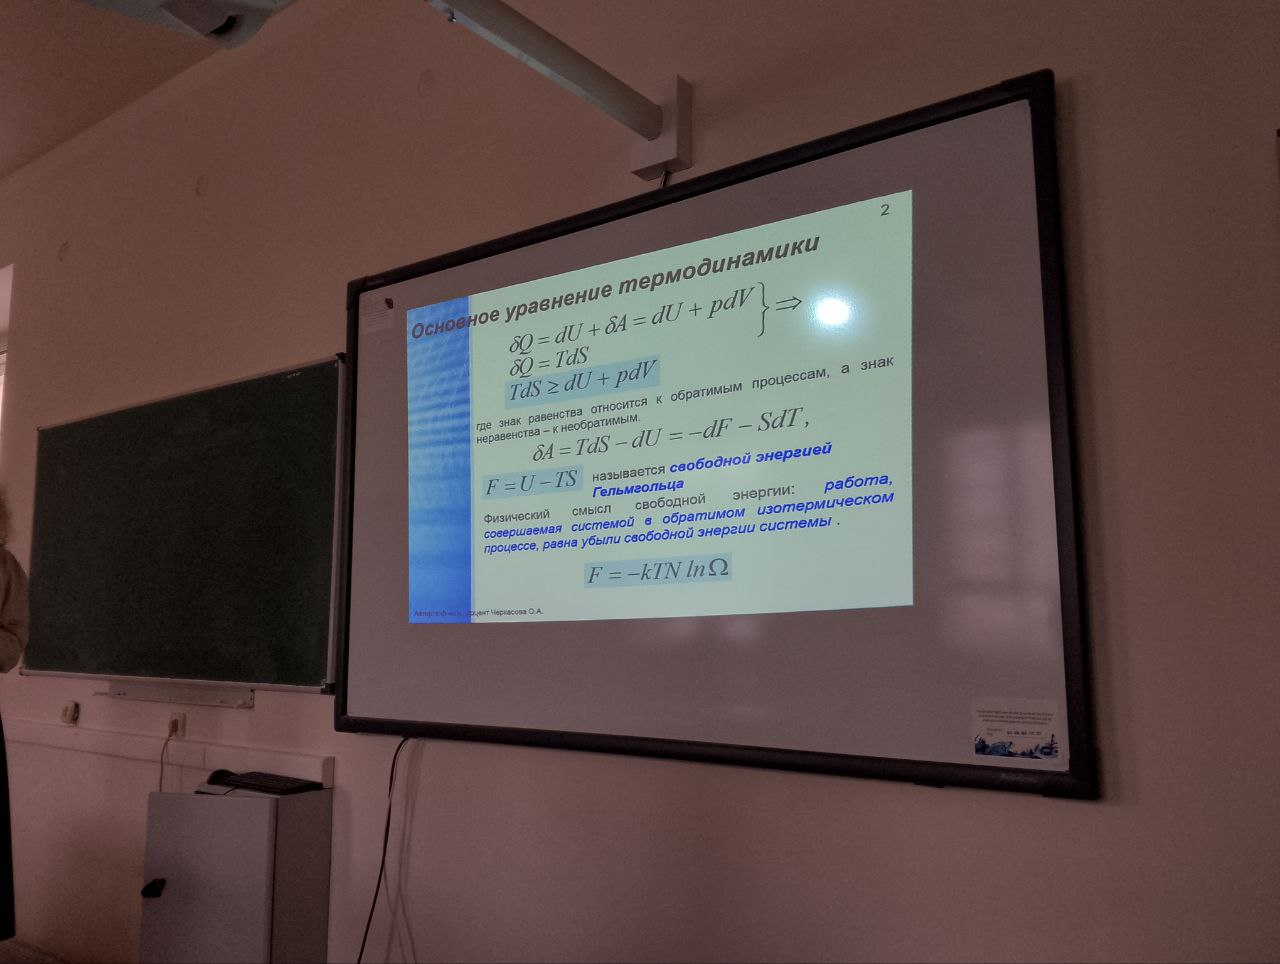
\includegraphics[width=\textwidth]{1.jpg}
\end{figure}
\section{Термодинамические потенциалы}
\begin{figure}[H]
    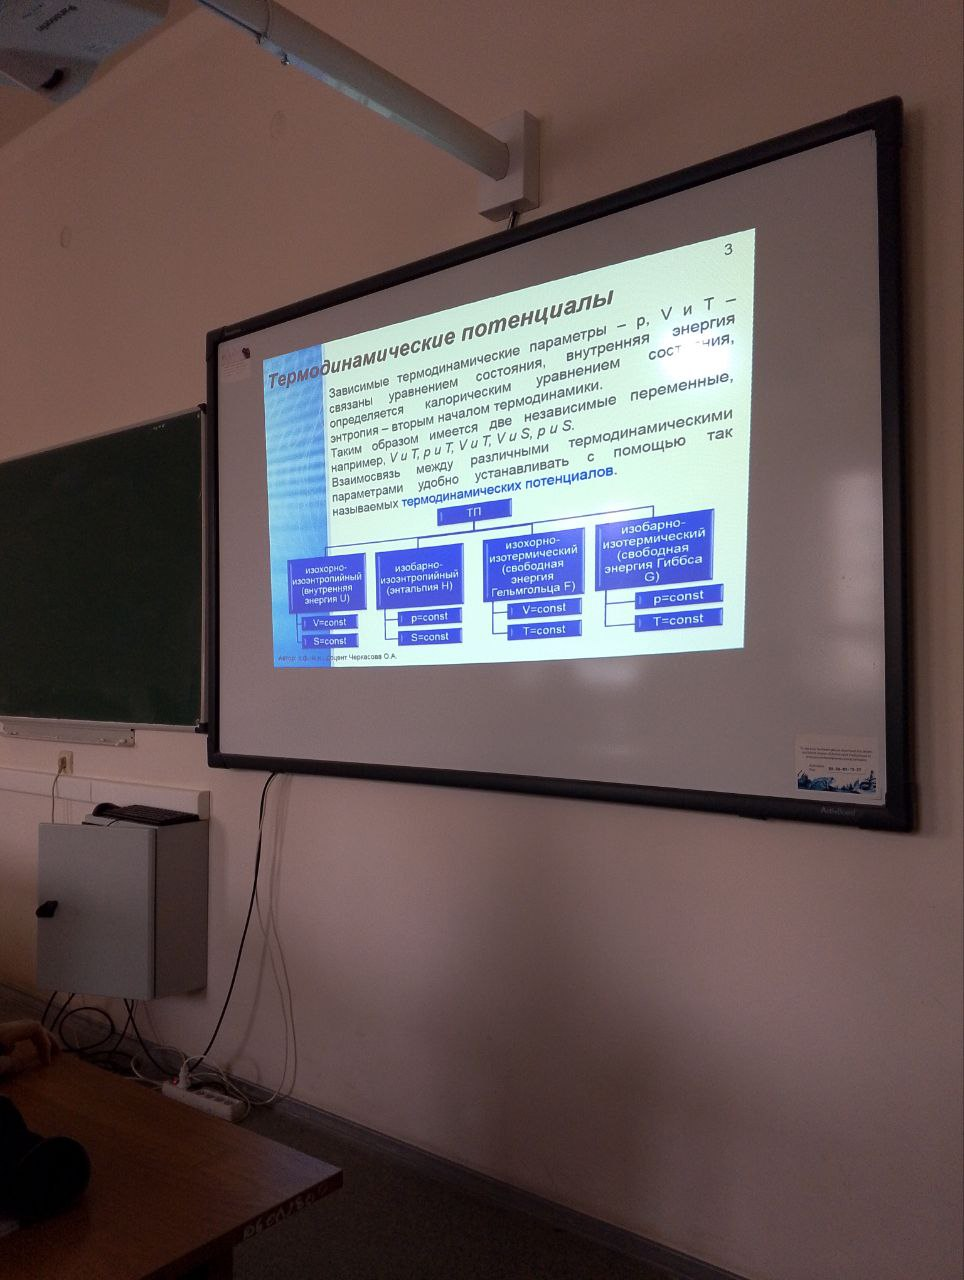
\includegraphics[width=\textwidth]{2.jpg}
\end{figure}
\begin{figure}[H]
    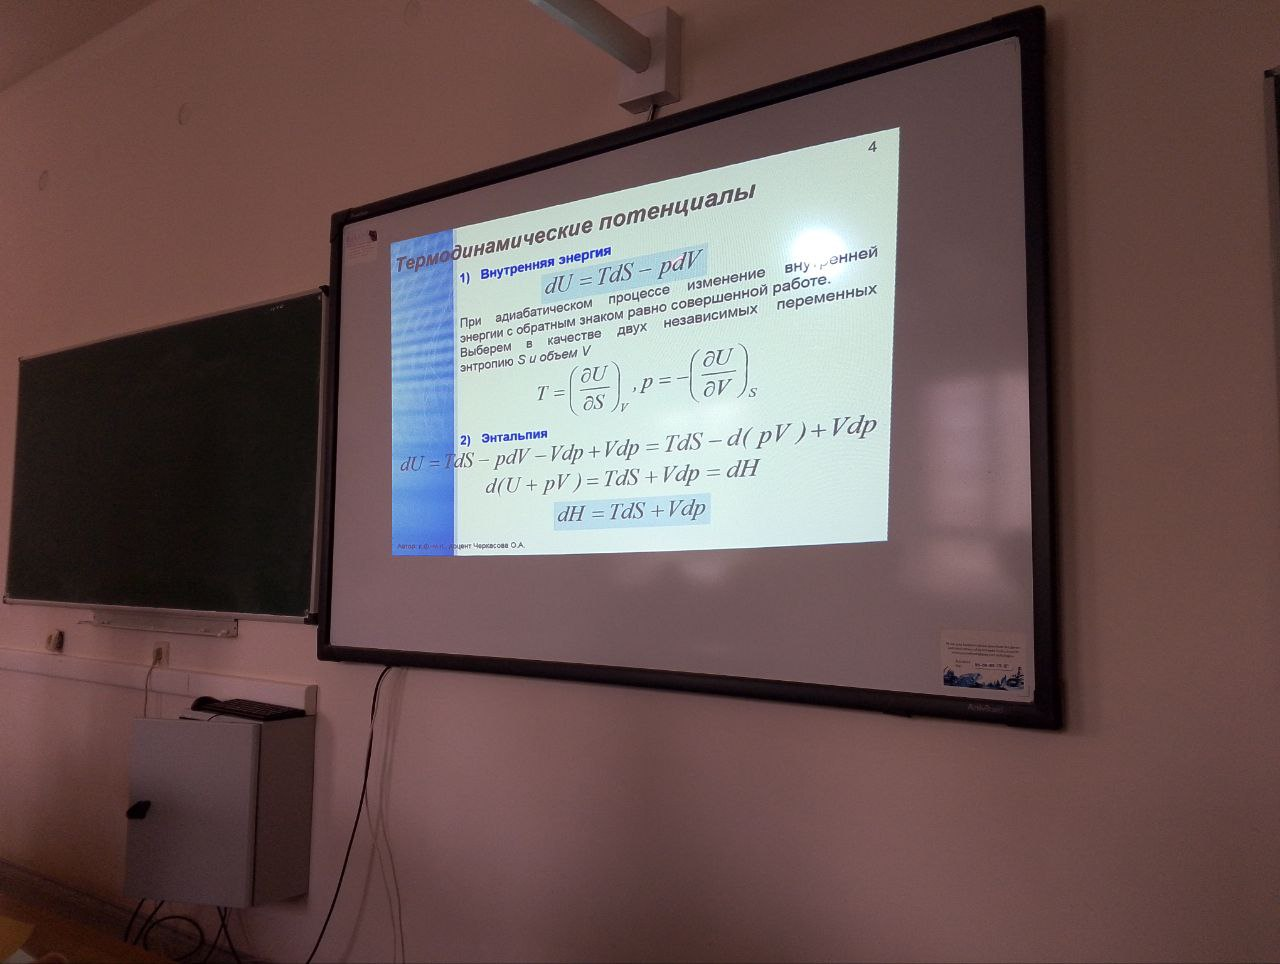
\includegraphics[width=\textwidth]{3.jpg}
\end{figure}

Исходя из этого, мы видим, что у нас естественными параметрами будут непосредственно энтальпия и наше давление. Температура и объём --- частные производные от эльтальпии. Эльтальпия отвечает за всевозможный переброс тепла внутри термодинамической системы.

\begin{figure}[H]
    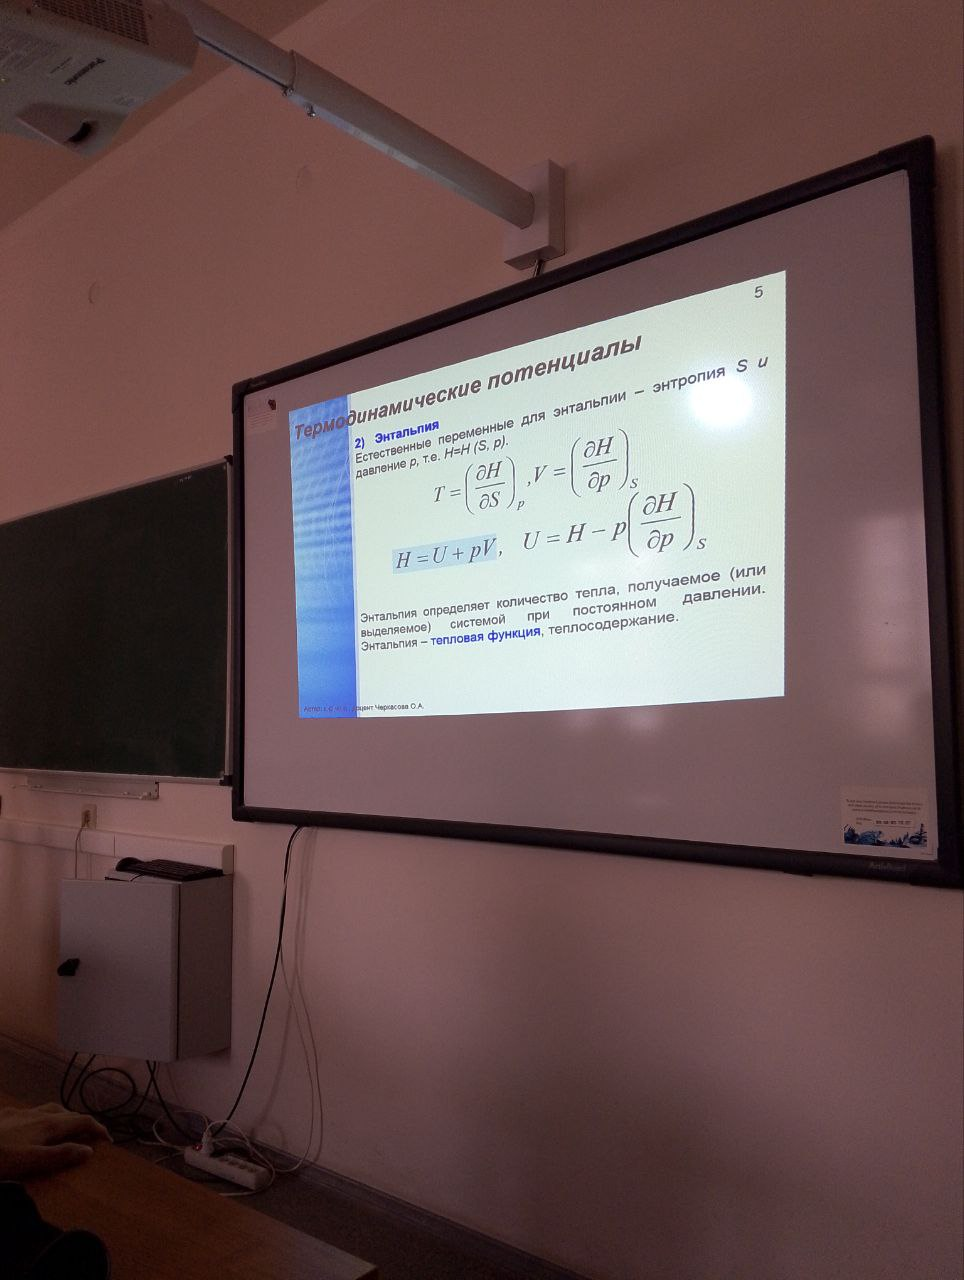
\includegraphics[width=\textwidth]{4.jpg}
\end{figure}

\begin{figure}[H]
    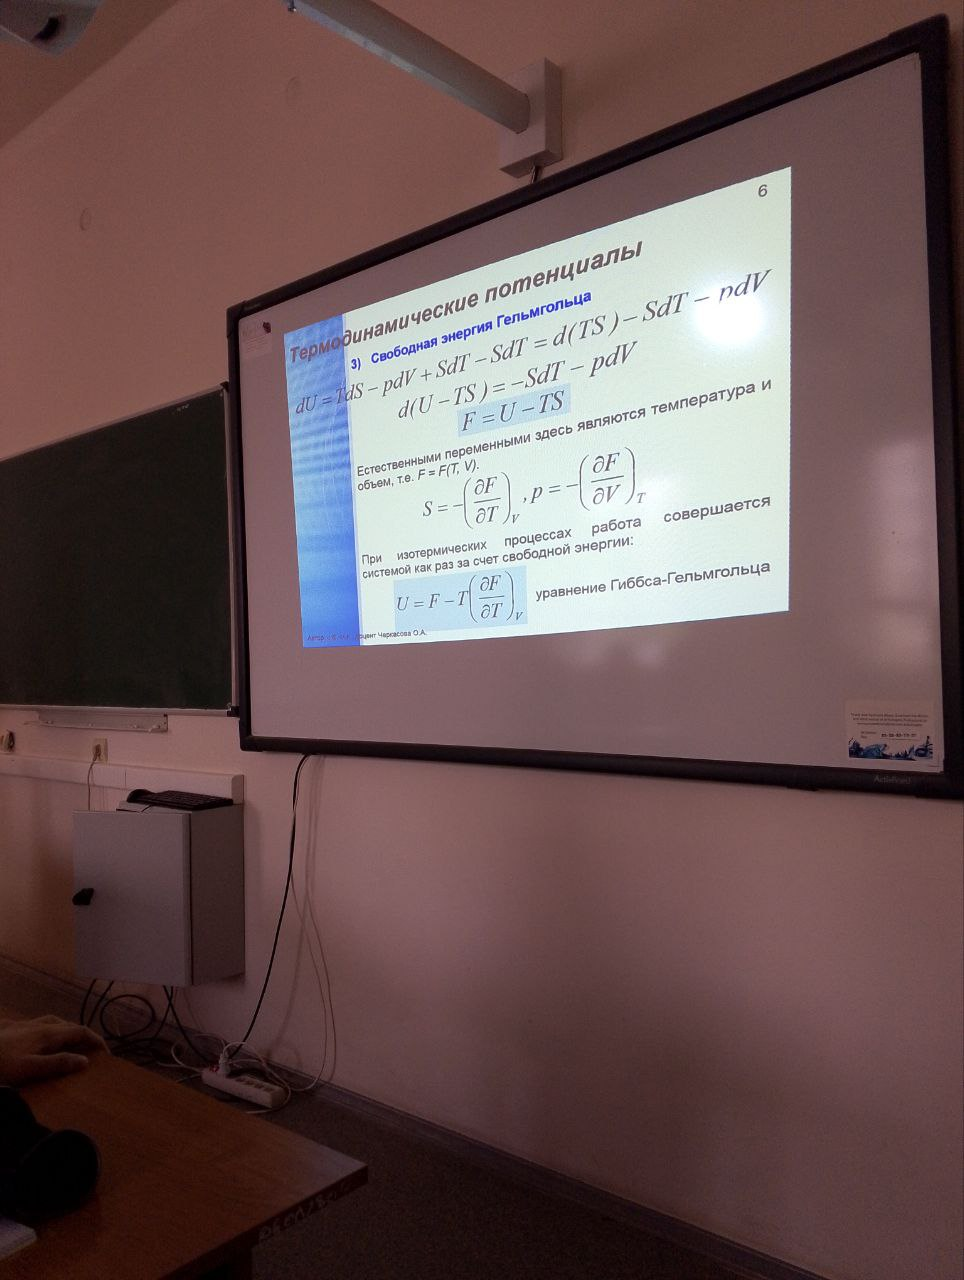
\includegraphics[width=\textwidth]{5.jpg}
\end{figure}

\begin{figure}[H]
    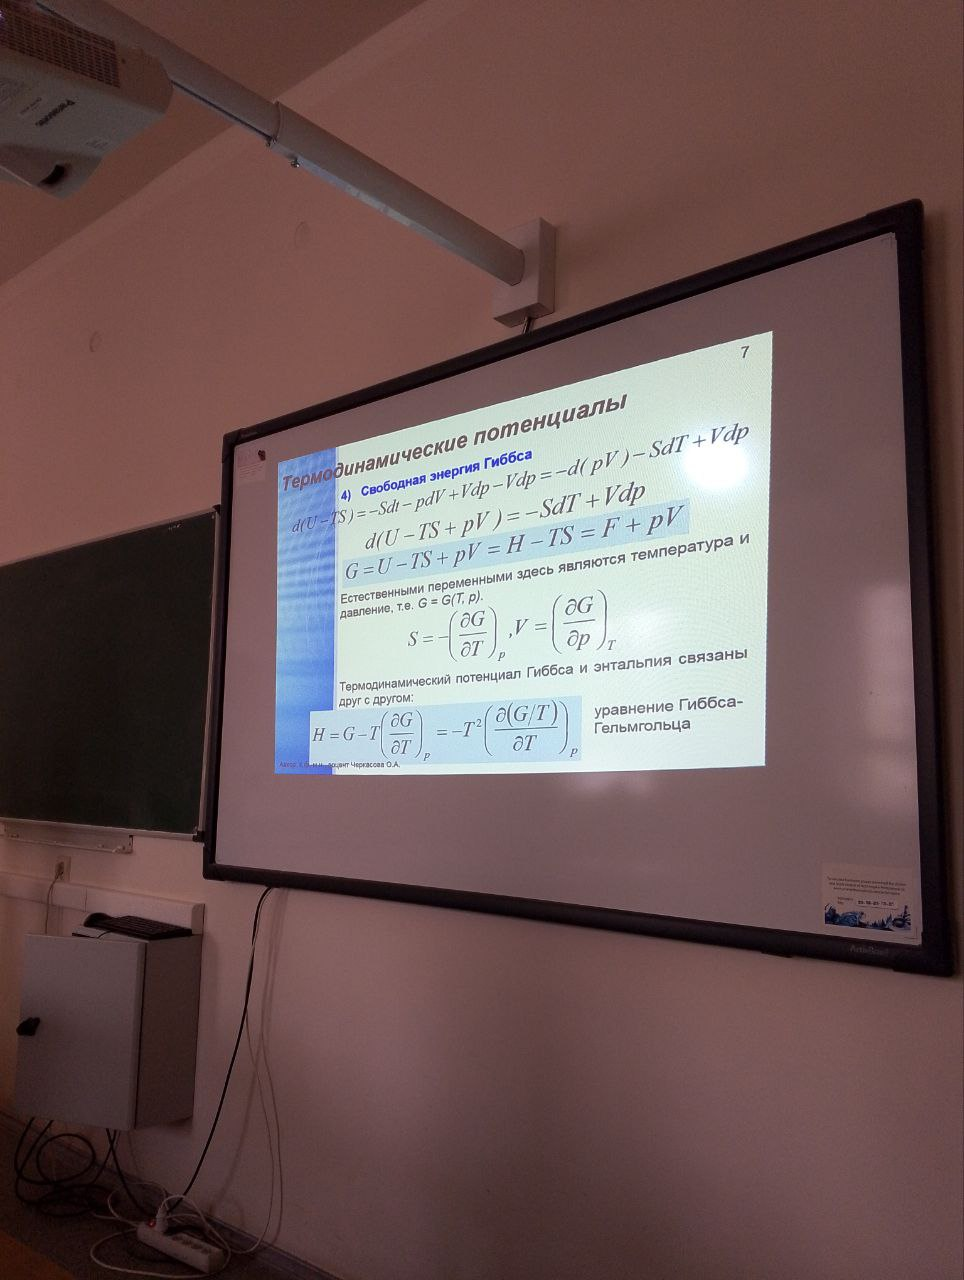
\includegraphics[width=\textwidth]{6.jpg}
\end{figure}
Здесь не $t$,а$T$ (опечатка)

\begin{figure}[H]
    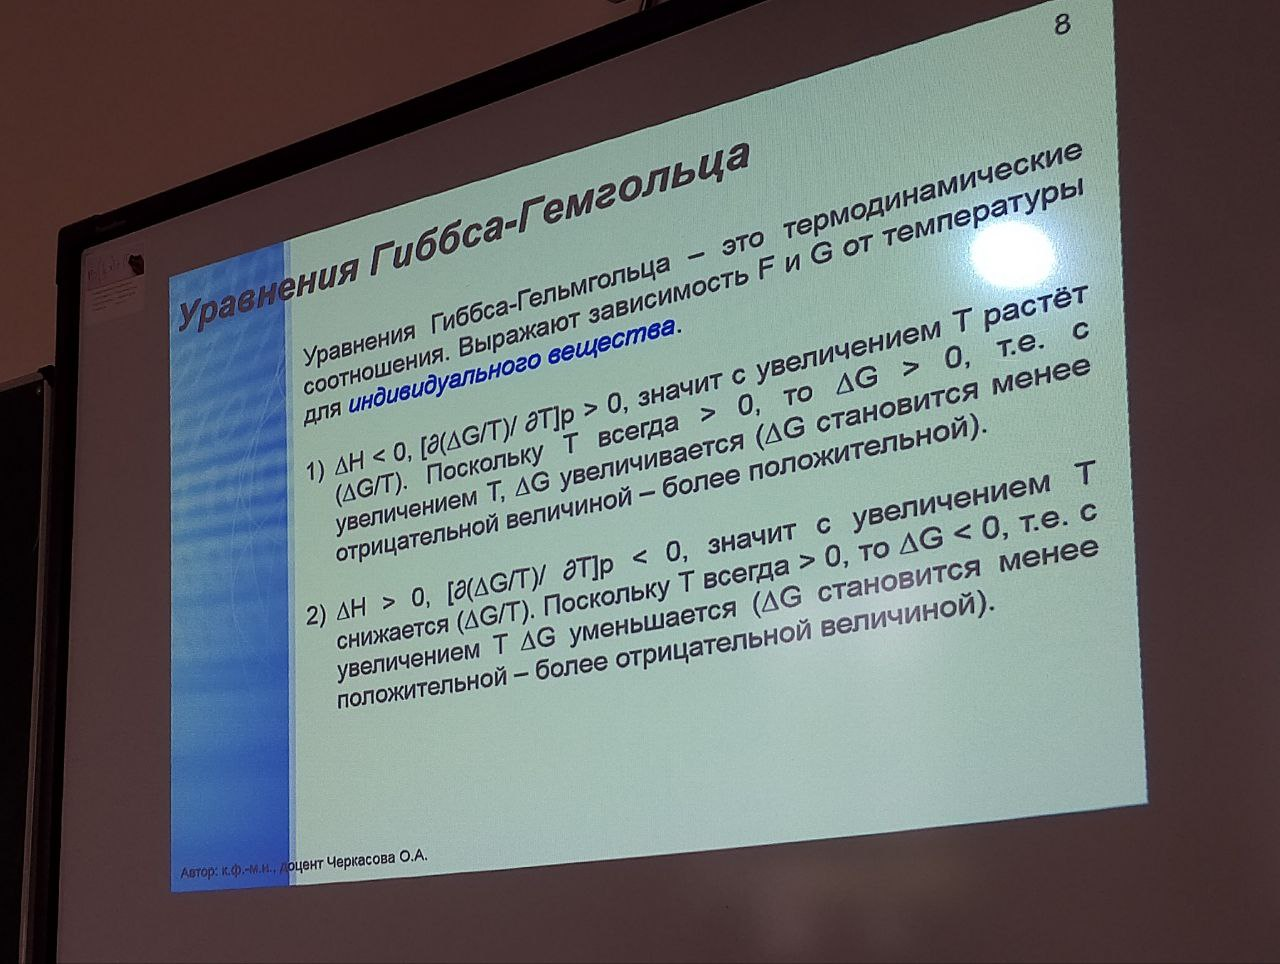
\includegraphics[width=\textwidth]{7.jpg}
\end{figure}
\par Отношение к температуре всегда будет расти. 

\begin{figure}[H]
    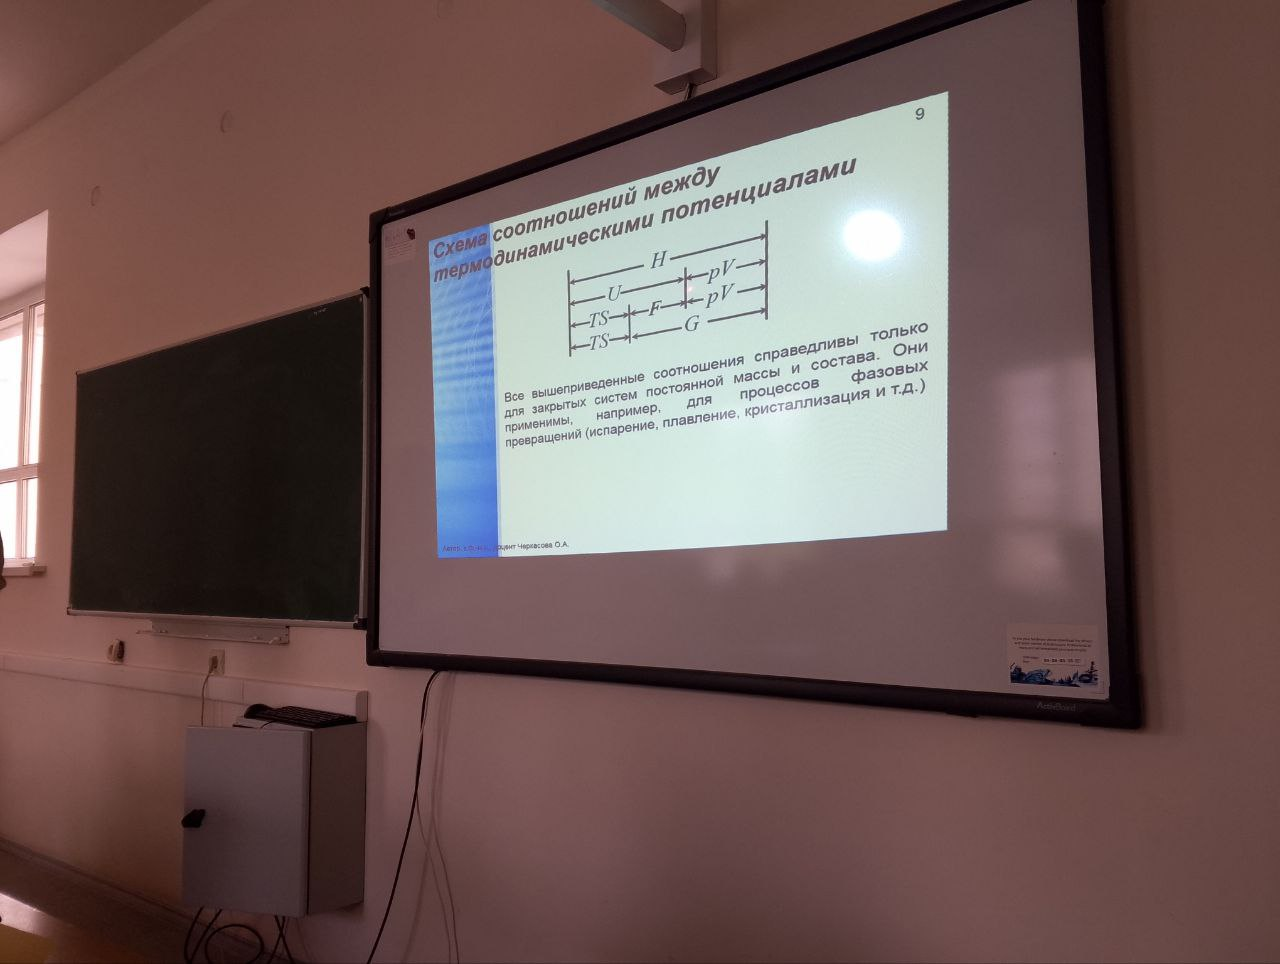
\includegraphics[width=\textwidth]{8.jpg}
\end{figure}

\begin{figure}[H]
    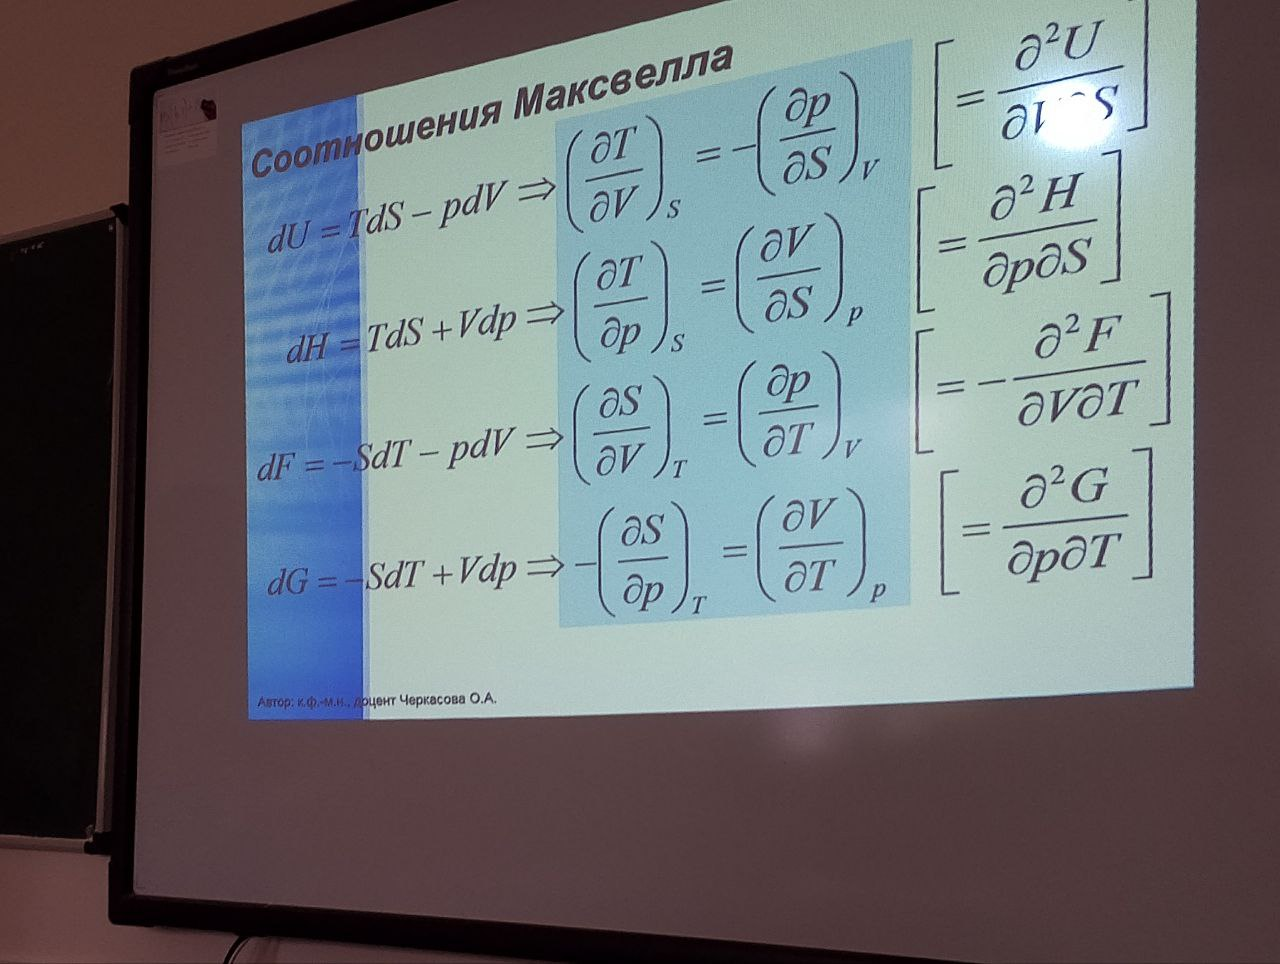
\includegraphics[width=\textwidth]{9.jpg}
\end{figure}

\begin{figure}[H]
    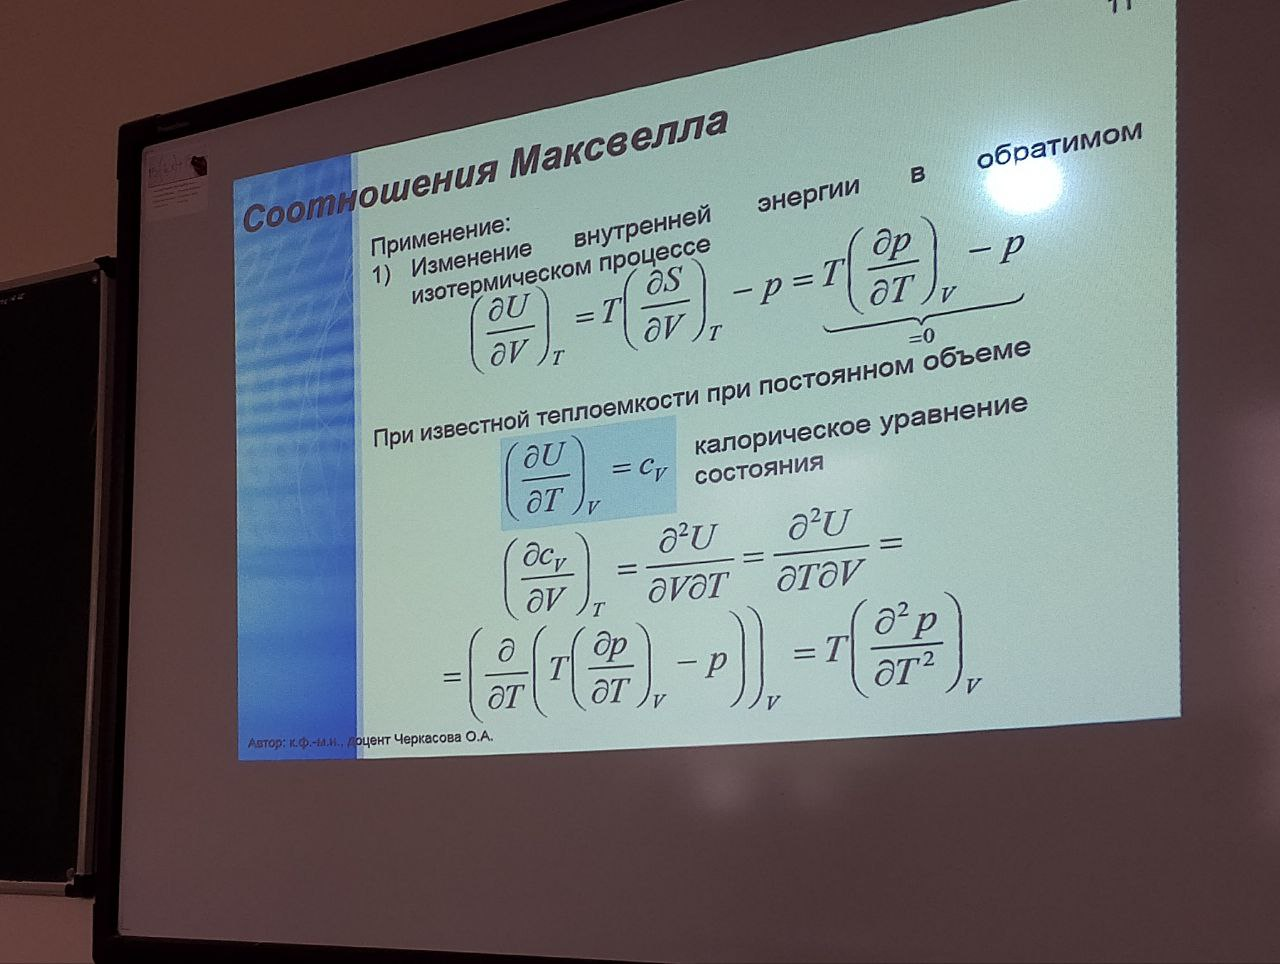
\includegraphics[width=\textwidth]{10.jpg}
\end{figure}
С помощью этих уравнений мы можем получить колорическое уравнение состояния.

Подставляя наше уравнение в уравнение Максвелла, мы в конечном итоге получаем, что изменение теплоёмкости при постоянном объёме в системе с постоянной температурой будет определяться второй производной от давления при температуре и постоянном объёме.
\begin{figure}[H]
    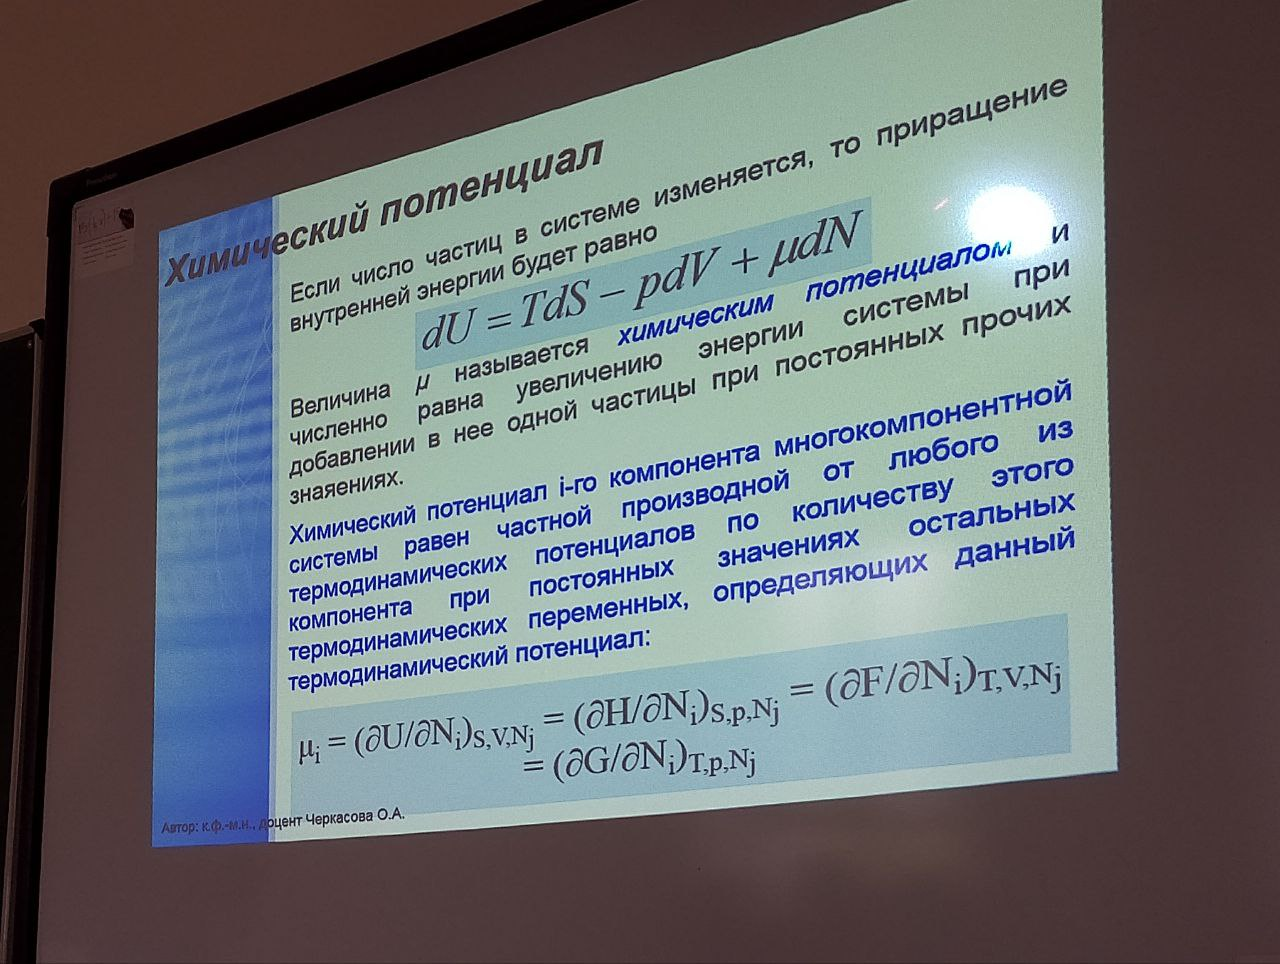
\includegraphics[width=\textwidth]{12.jpg}
\end{figure}

\begin{figure}[H]
    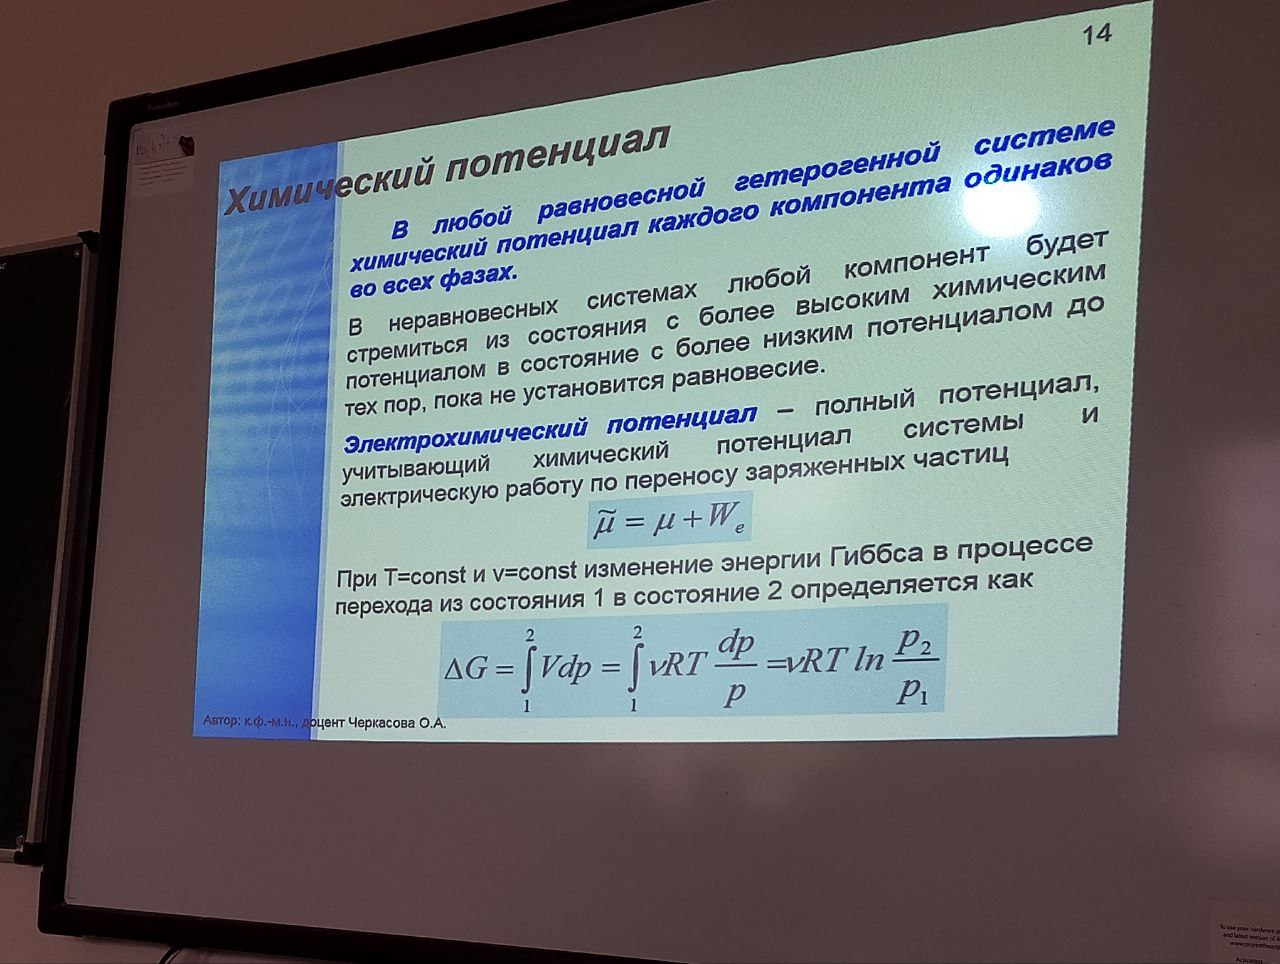
\includegraphics[width=\textwidth]{13.jpg}
\end{figure}
Если у нас рассматриваются неравновесные процессы (нелинейная физика),  у нас будет наблюдаться градиент физического потенциала. У нас будет происходить процесс диффузии. Отсюда, с учётом природы этих веществ (не всегда они будут электрически нейтральными), у нас появляется электрохимический потенциал. Он учитывает химические процессы и электрическую работу, которую будут затрагивать компоненты системы для перехода себя из одного положения в другое.

Если $T$ и количество вещества $\nu$ не изменяются, см. нижнюю формулу.

электрохимический потенциал определяет направление движения электрических зарядов внутри материала. Это способствует протеканию тока внутри материала.

\begin{figure}[H]
    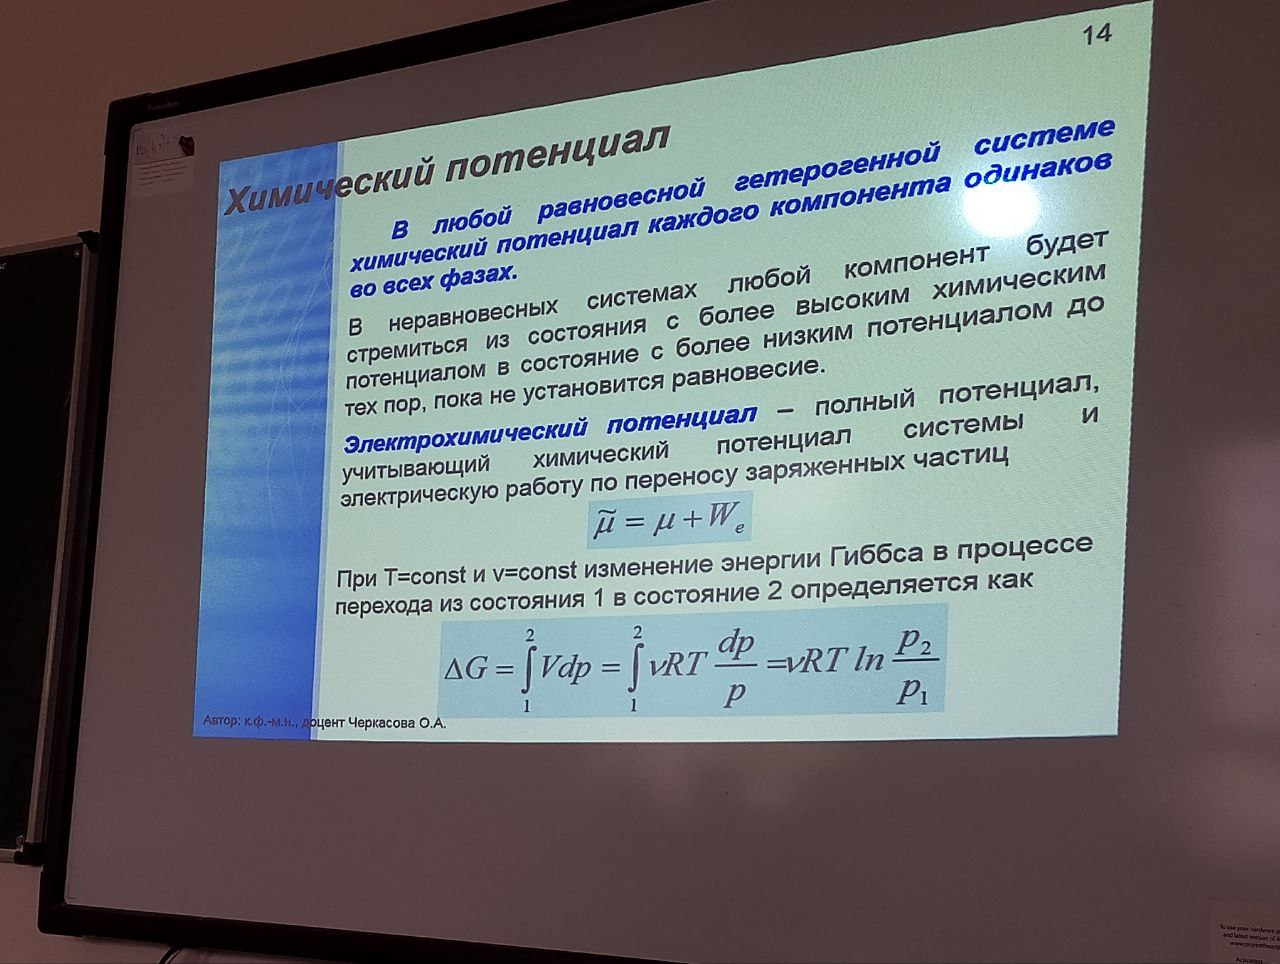
\includegraphics[width=\textwidth]{14.jpg}
\end{figure}
\end{document}